\documentclass{article}

\usepackage{tmlr}

\usepackage{hyperref}
\usepackage{url}
\usepackage{booktabs}
\usepackage{graphicx}
\usepackage{amsmath,amssymb}

\title{A Pre-Registered Refutation of Hierarchical Credit Sharing for Disruption Recovery in Non-Stationary Structured Bandits\thanks{A large language model was used as a writing assistant. All numerical claims were checked against frozen artifacts; the hypotheses, estimand, and confirmatory result were not generated by the model.}}

\author{Anonymous authors}

\newcommand{\rrt}{\mathrm{RRT}}
\newcommand{\deltaRRT}{\delta_{\rrt}}

\begin{document}
\maketitle

\begin{abstract}
A pre-registered, frozen comparison found that the tested hierarchical routing update did not improve disruption recovery relative to the edge-only comparator under the frozen V1 configuration, and the pre-specified negative-transfer safety criterion was not satisfied.
On $n=97$ paired synthetic scenarios at shared-shock fraction $\rho=0.50$, mean restricted recovery time was $42.1\%$ \emph{higher} for the fixed hierarchical routing update than for edge-only adaptation (bootstrap $95\%$ interval $+11.9\%$ to $+79.1\%$; one-sided upper bound $+72.1\%$).
The frozen analysis plan therefore classifies the primary hypothesis as \textbf{REFUTED}.
At $\rho=0$, the one-sided upper bound $+16.3\%$ exceeds the pre-specified non-inferiority margin $+10\%$, so the negative-transfer safety gate also fails.
This paper reports that terminal result without narrative rescue.
Post-confirmatory diagnostics, which are not confirmatory evidence, show (i)~a $1.72\times$ inflation of paired-difference dispersion from a $20$-pair pilot to the confirmatory sample, (ii)~an equalization-triage finding of class EQ-B: the two methods shared nominal temperature and exploration probability but induced materially different warm-up action distributions, and (iii)~no detectable sharing advantage on restricted recovery time even at the $\rho=1$ diagnostic cell, while dynamic regret remained worse for hierarchical pooling.
The result is bounded by the tested graph, observation contract, shock construction, and parameter range.
It does not establish a causal mechanism, a crossover $\rho^\star$, or external validity.
\end{abstract}

\section{Introduction}

Adaptive routing systems are often motivated by a structural hypothesis: if a disruption is shared across related actions, then sharing credit through a coarser representation should accelerate recovery relative to purely local updates.
That hypothesis is testable.
It is also easy to overclaim.

This paper reports a pre-registered confirmatory experiment, protocol MG-EXP-V1, that compared a hierarchical node-edge credit-sharing learner with an edge-only adaptor on a non-stationary combinatorial semi-bandit.
The scientific object is the implemented comparison, not a metaphor.
``Mycelial'' is a software name; the paper does not study mycelial intelligence.

The frozen primary estimand is the relative difference in mean restricted recovery time,
\[
\deltaRRT
=
\frac{\mathbb{E}[\rrt_{\mathrm{hier}}]-\mathbb{E}[\rrt_{\mathrm{edge}}]}{\mathbb{E}[\rrt_{\mathrm{edge}}]},
\]
at $\rho=0.50$, with $\rrt=\min(\text{recovery time},\tau)$ and $\tau=300$ post-shock steps.
Negative values mean faster hierarchical recovery.
The confirmatory decision used a paired bootstrap, one-sided $95\%$ upper bound, and a pre-specified relevant benefit of $-20\%$.
A separate safety gate at $\rho=0$ tested non-inferiority against margin $\Delta_{\mathrm{NI}}=+0.10$.

The experiment reached a legitimate terminal state: \textbf{REFUTED}, and the safety gate failed.
That status applies to the complete frozen policy mechanism, not to hierarchical representation in isolation.
A post-confirmatory equalization audit identified a material effective-policy mismatch (class EQ-B), limiting attribution of the observed difference to hierarchical representation alone.
A negative result that remains unpublished does not capitalize the work that produced it.
We therefore report the frozen test and the strongest interpretation the artifacts support, and we keep every mechanistic story in a labelled diagnostic section.

\paragraph{What this paper does not claim.}
It does not claim that hierarchical pooling fails universally.
It does not claim that adaptive pooling was tested.
It does not claim that a crossover exists.
It does not claim that fixed pooling \emph{caused} the failure.
One candidate explanation is structural-prior misspecification induced by fixed pooling; another is that the compared methods did not operate at equalized effective policy scale.
Those remain candidate explanations.

\section{Related work}

Non-stationary bandits study tracking under changing rewards, including switching and variation-budget models \citep{garivier2011switching,besbes2014nonstationary,russac2019weighted}.
Classical stochastic bandits isolate exploration--exploitation without structure \citep{auer2002finite}.
Combinatorial and semi-bandit models add a path or subset action \citep{cesabianchi2012combinatorial,chen2013combinatorial,kveton2015tight}.
Shrinkage and hierarchical Bayes reduce variance by sharing strength \citep{james1961estimation,gelman2013bayesian}.
Hierarchical Thompson sampling and related partial-pooling bandits apply that idea online \citep{russo2018tutorial,hong2022hierarchical}.
When several representations or algorithms are available, master algorithms such as CORRAL and regret balancing treat model selection as the object \citep{agarwal2017corralling,pacchiano2020model}.
Misspecification is a first-class failure mode of structured models \citep{lattimore2020bandit}.

This paper is not a new algorithm paper.
It is a pre-registered comparison of one fixed hierarchical sharing rule against edge-only adaptation under a frozen recovery estimand.
Adaptive pooling, empirical-Bayes shrinkage, and master algorithms are related, and they were \emph{not} the V1 treatments.
Reproducibility practice \citep{pineau2021improving} is part of the contribution only insofar as the freeze, seed populations, claim boundary, and sealed artifacts make the negative result inspectable.

\section{Experimental design}

\subsection{Environment}
The environment is a layered directed acyclic graph with three internal layers and three alternatives per layer ($27$ source-to-sink paths).
At each step a method selects one path and observes local rewards on traversed edges only.
A single shock occurs after $200$ warm-up steps.
The shock has constant $\ell_2$ magnitude $m=0.55$ and shared-node fraction $\rho$:
\[
d(\rho)=-m\bigl(\sqrt{\rho}\,n+\sqrt{1-\rho}\,i\bigr),
\]
where $n$ is a unit node-incidence pattern and $i$ is a disjoint unit edge-interaction pattern.
The grid is $\rho\in\{0,0.25,0.50,0.75,1\}$.
Only $\rho=0.50$ (primary) and $\rho=0$ (safety) are confirmatory.
$\rho=1$ is a pre-specified diagnostic construct check.
Other $\rho$ values are exploratory.

Scenarios are immutable and paired: every method faces identical potential outcomes.
Environment and agent random streams are isolated.
Pre- and post-shock optima are certified before a scenario is admitted.

\subsection{Methods}
Edge-only adaptation maintains a clipped conductance per edge, with temporal decay, local updates, softmax temperature $T=0.20$, and basal exploration probability $\epsilon=0.08$.
Hierarchical pooling uses the additive score
\[
\mathrm{score}(e=(u,v),t)=\mathrm{base}+a_{u,t}+b_{v,t}+c_{e,t}
\]
with sum-to-zero projection and shrinkage.
It uses the same $T$ and $\epsilon$, but different learning rates, an unbounded score, and projection.
Node-only ablation and a structured sliding-window UCB baseline are secondary; they cannot support the confirmatory claim.

\subsection{Estimand, freeze, and decision rule}
Restricted recovery time uses a trailing window of $10$ steps, a confirmation window of $20$ steps, and a $90\%$ oracle-utility threshold.
Administrative censoring sets unrecovered trials to $\tau=300$.
The primary test is $H_0:\deltaRRT\ge 0$ versus $H_1:\deltaRRT<0$ at $\rho=0.50$.
The safety gate is $H_0:\deltaRRT\ge +0.10$ versus $H_1:\deltaRRT<+0.10$ at $\rho=0$.
The confirmatory family contains one superiority hypothesis, so no multiplicity split is required.
Result states $\mathrm{SUPPORTED}$, $\mathrm{CONDITIONAL}$, $\mathrm{INCONCLUSIVE}$, $\mathrm{REFUTED}$, and $\mathrm{PROTOCOL\_INVALID}$ were frozen before any confirmatory outcome was observed.
$\mathrm{REFUTED}$ occurs when the one-sided upper bound is not below zero \emph{and} the two-sided interval excludes the relevant benefit $-0.20$.

The protocol, analysis plan, configuration hash, and confirmatory seed file were bound before execution.
$N=97$ is the unfiltered prefix of a precommitted pool.
No post-pilot tuning of hyperparameters, estimand, or thresholds occurred.

\subsection{Pilot and sample size}
A disjoint $20$-seed pilot was used only to estimate paired variance for a normal-approximation sample-size formula (one-sided $\alpha=0.05$, power $0.80$, design target $\deltaRRT=-0.20$).
The pilot primary point estimate was $-10.2\%$ with one-sided upper bound $+21.9\%$, and the $\rho=0$ gate already failed (upper bound $+18.0\%$).
Those numbers are recorded, not hidden, and they are not confirmatory evidence.

\section{Why the protocol was not changed after the pilot}

A reviewer may ask: the pilot already produced an unfavourable or non-conclusive signal and failed the safety gate; why was the protocol not changed before confirmation?

The pilot population was defined in advance.
Its purpose was variance and sample-size estimation, not hypothesis revision.
Pilot and confirmatory populations were disjoint.
Pilot evidence was not permitted to redefine the hypothesis, estimand, $\rho$ grid, methods, or decision thresholds.
Changing the protocol after observing an unfavourable pilot signal would defeat the freeze.
Confirmatory execution therefore proceeded under the frozen protocol.
That is methodological discipline, not a weakness to hide.

\section{Confirmatory results}

\paragraph{Primary contrast ($\rho=0.50$, hierarchical vs edge-only).}
Mean restricted recovery time was $51.18$ for the fixed hierarchical routing update and $36.01$ for the edge-only comparator, so $\widehat{\deltaRRT}=+42.1\%$
(bootstrap $95\%$ interval $+11.9\%$ to $+79.1\%$; one-sided upper bound $+72.1\%$; $10{,}000$ resamples; $n=97$).
The relevant benefit $-20\%$ lies outside the interval.
The frozen mapping therefore returns \textbf{REFUTED}.

\paragraph{Safety gate ($\rho=0$).}
$\widehat{\deltaRRT}=+1.5\%$, one-sided upper bound $+16.3\%$ against margin $+10\%$.
Non-inferiority is not established: $\mathrm{NEGATIVE\_TRANSFER\_NOT\_EXCLUDED}$.

\paragraph{Integrity.}
$97/97$ primary pairs executed.
Non-administrative censoring: $0$.
Method failures inside frozen contrasts: $0$.
Censoring, where present, is administrative restriction at $\tau=300$.

These statements are $\mathrm{FROZEN\_CONFIRMATORY}$.
Exploratory rows at other $\rho$ values, node-only comparisons, and SW-UCB comparisons are reported in the sealed artifact and are not inferential claims.

\section{Post-confirmatory diagnostics}

Every analysis in this section is labelled $\mathrm{POST\_CONFIRMATORY\_DIAGNOSTIC}$.
Diagnostics may explain $\mathrm{REFUTED}$; they may never overwrite $\mathrm{REFUTED}$.

\subsection{Pilot-to-confirmatory variance}
The empirical paired difference $\rrt_{\mathrm{hier}}-\rrt_{\mathrm{edge}}$ at $\rho=0.50$ has mean $-4.2$ and SD $32.52$ in the pilot ($n=20$), versus mean $+15.16$ and SD $55.95$ in the confirmatory sample ($n=97$).
The confirmatory-to-pilot SD ratio is $\mathbf{1.72\times}$.
A previously discussed factor of $4.54\times$ does not reproduce from current artifacts and is not reported.

The confirmatory paired-difference distribution is right-skewed (skewness $1.63$), with median $+6$ against mean $+15.16$, range $[-78,+250]$, and $6/97$ pairs flagged by a $3\times\mathrm{MAD}$ rule.
Removing those pairs reduces SD from $55.95$ to $37.49$.
Signs are mixed: $54.6\%$ of pairs have hierarchical slower, $44.3\%$ faster.
The ratio-of-means estimand ($+42.1\%$) is therefore not a near-uniform delay.

The $20$-pair pilot provided an unstable variance estimate in this environment.
That is a methodological limitation of the sample-size design, not a reason to discard the confirmatory result.
Future protocols, including any V1.5 study, should not rely on a normal approximation from a small pilot unless a bootstrap or simulation-based procedure supports it.

\begin{figure}[t]
\centering
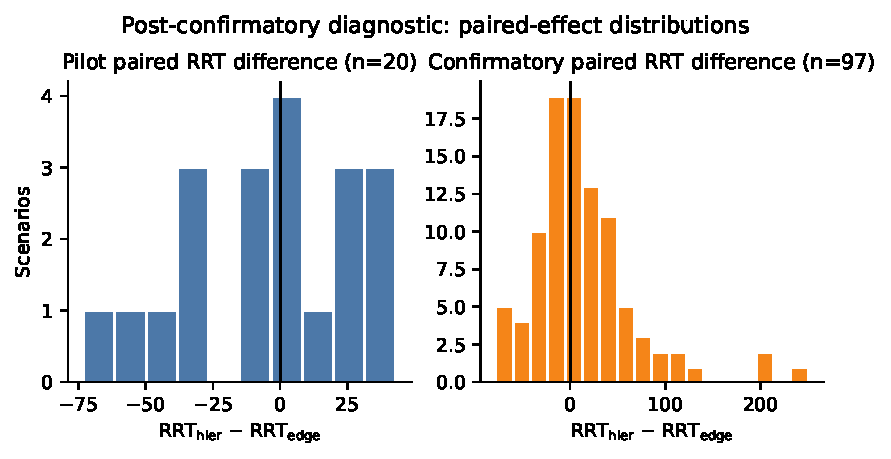
\includegraphics[width=\linewidth]{figures/paired_differences.pdf}
\caption{Paired RRT differences at $\rho=0.50$. Left: pilot ($n=20$), $\mathrm{PILOT\_EVIDENCE\_NOT\_CONFIRMATORY}$. Right: confirmatory ($n=97$), $\mathrm{POST\_CONFIRMATORY\_DIAGNOSTIC}$ distribution of the frozen primary pairs. Positive values mean slower hierarchical recovery.}
\label{fig:paired}
\end{figure}

\subsection{Censoring and $\tau=300$}
All recorded censoring is administrative.
At the primary cell, $0/97$ edge-only trials and $1/97$ hierarchical trials are restricted at $\tau$.
The $1.0$ percentage-point gap cannot account for a $+42.1\%$ relative-mean effect.
SW-UCB shows substantially more administrative censoring at several exploratory $\rho$ values; those rows have no error control.
Restricted recovery time remains a thresholded functional: this paper does not replace it with a new primary outcome.

\subsection{Equalization triage}
Parameter parity is not policy parity.
The two confirmatory arms shared code paths for routing, the same nominal temperature $T=0.20$, the same $\epsilon=0.08$, and the same local-feedback contract.
They did not share update geometry: edge-only scores are clipped conductances, while hierarchical scores are unbounded additive effects with projection.

Using stored decision traces, we measured realized warm-up action distributions (first $200$ steps) at $\rho=0.50$:
\begin{itemize}
\item path entropy as a fraction of $\log 27$: $0.629$ (edge-only) vs $0.969$ (hierarchical);
\item max path probability: $0.468$ vs $0.076$;
\item selected-score standard deviation ratio: $12.08$;
\item exploration-step rates: $0.224$ vs $0.221$ (gap $0.003$);
\item optimal-pre-path rates: $0.136$ vs $0.043$ (gap $0.094$).
\end{itemize}
Pre-declared tolerances classified this as \textbf{EQ-B}: material limitation, result still interpretable.
Both arms remain non-degenerate; hierarchical warm-up is near-diffuse rather than collapsed.
The frozen comparison is therefore a comparison of the \emph{implemented methods}, not a clean isolation of representation.
We revise the manuscript claim accordingly and still submit the $\mathrm{REFUTED}$ outcome.
This is not $\mathrm{EQ\text{-}C}$: we do not treat the primary comparison as scientifically uninterpretable, and we do not erase the refutation.

\begin{figure}[t]
\centering
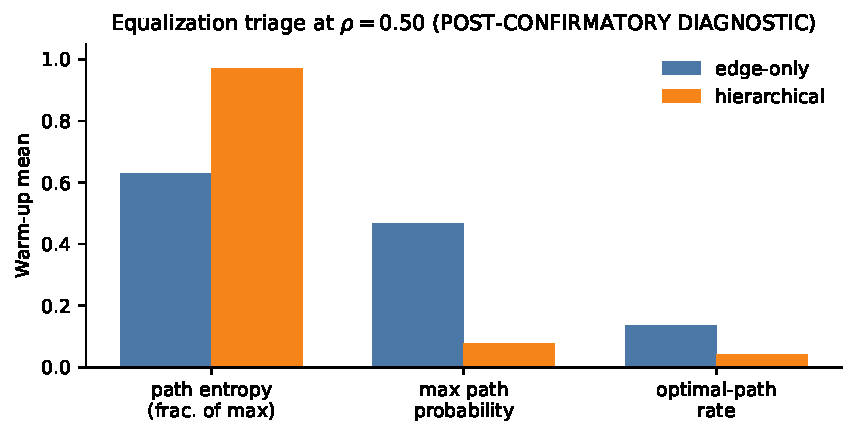
\includegraphics[width=\linewidth]{figures/equalization_warmup.pdf}
\caption{Warm-up realized-action summaries at $\rho=0.50$. Status: $\mathrm{POST\_CONFIRMATORY\_DIAGNOSTIC}$. Stored traces contain selected scores, not the full candidate-score vector; entropy and concentration are computed from realized paths.}
\label{fig:eq}
\end{figure}

\subsection{Dynamic range and regret divergence}
On the frozen $\rho$ grid, hierarchical mean RRT is better only at the $\rho=1$ diagnostic cell ($\widehat{\deltaRRT}=-8.9\%$; interval $-27.0\%$ to $+14.6\%$; one-sided upper bound $+10.2\%$, which is not below zero).
That is not a detectable sharing advantage under the frozen one-sided rule.
At the same cell, relative dynamic regret is $+79.9\%$ \emph{against} hierarchical pooling.
Restricted recovery time and dynamic regret therefore disagree in sign at $\rho=1$ and agree (both against hierarchical pooling) at $\rho\in\{0,0.25,0.50,0.75\}$.
Dynamic regret is \emph{not} retrofitted as a V1 primary endpoint.
For future studies it is a candidate co-primary, with its own estimand, power, and multiplicity control.

Failure at $\rho=1$ to produce a clear sharing advantage is compatible with at least three explanations: an implementation defect, weakness of the sharing mechanism, or insufficient environmental dynamic range.
This diagnostic cannot separate them.
No additional $K_{\mathrm{edge}}/K_{\mathrm{node}}$, shock-magnitude, or noise factorial was run before submission; those sweeps belong to a later protocol and would use reserved disjoint seeds.

\begin{figure}[t]
\centering
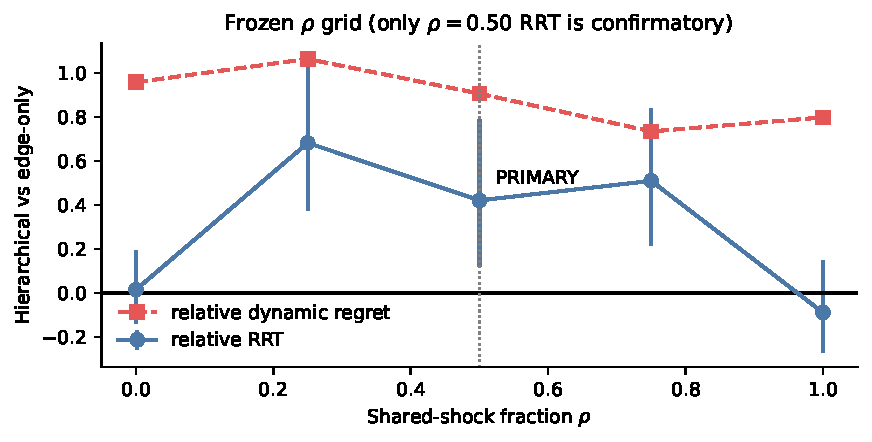
\includegraphics[width=\linewidth]{figures/rho_grid_diagnostic.pdf}
\caption{Relative hierarchical-versus-edge-only effects across the frozen $\rho$ grid. Only $\rho=0.50$ restricted recovery time is confirmatory. All other points are exploratory or diagnostic.}
\label{fig:rho}
\end{figure}

\subsection{Falsification capacity of the simulator}
The frozen apparatus produced a strongly unfavourable result for the target mechanism.
That demonstrates falsification capacity and weakens the simplistic objection that the simulator was mechanically designed so that hierarchical pooling must win.
It does not imply that the simulator is unbiased, and it does not disprove simulator-bias threats.
Those threats remain in Section~\ref{sec:threats}.

\section{Threats to validity}
\label{sec:threats}

The strongest threats are listed first.
\begin{itemize}
\item \textbf{Synthetic environment.} No real-provider traces were used. External validity is $\mathrm{UNSUPPORTED}$.
\item \textbf{Effective-policy mismatch (EQ-B).} Nominal hyperparameter equality did not yield equalized action distributions. Attribution of the V1 performance difference to hierarchical representation alone is unsupported; effective policy scale was not equalized in the frozen comparison. Mechanistic attribution to ``hierarchy'' is limited. The frozen result remains $\mathrm{REFUTED}$ for the complete tested mechanism.
\item \textbf{Limited dynamic range.} Even at $\rho=1$, restricted recovery time does not detect a sharing advantage under the frozen one-sided rule.
\item \textbf{Shock construction.} Constant $\ell_2$ magnitude with a single node pattern and a single interaction edge may not match other disruption models.
\item \textbf{Small pilot and variance instability.} $N=97$ used a normal approximation on $20$ pairs; confirmatory paired SD was $1.72\times$ larger.
\item \textbf{Thresholded outcome.} $\rrt$ censors at $\tau=300$ and depends on a $90\%$ trailing-window rule.
\item \textbf{Implementation fidelity.} Hierarchical scores, projection, and learning-rate split were frozen, not independently re-derived from a theorem.
\item \textbf{Hyperparameter and topology dependence.} One graph family, one temperature, one exploration rate.
\item \textbf{No independent reproduction.} All reproduction in this repository is internal and automated.
\item \textbf{No theorem.} Rate conjectures remain $\mathrm{CONJECTURE}$ / $\mathrm{OPEN\_PROBLEM}$.
\end{itemize}

\section{Reproducibility}

\subsection{Verification versus full reproduction}
Sealed confirmatory artifacts, configuration hash, seed-file hash, and the result state $\mathrm{REFUTED}$ are in the supplementary package.
The default command
\begin{verbatim}
python reproduce_confirmatory.py
\end{verbatim}
is verification and, when local raw trials already exist, reanalysis.
It checks freeze bindings and sealed hashes.
If \texttt{outputs/confirmatory/raw} is present it recomputes the frozen primary contrast from those files.
It does not recreate the $1940$ trials by itself.

The canonical full reproduction command is
\begin{verbatim}
python reproduce_confirmatory.py --full
\end{verbatim}
It re-executes the frozen experiment from frozen inputs ($97$ seeds $\times$ $5$ $\rho$ values $\times$ $4$ methods $= 1940$ trials), then analyzes, reports, and checks equality with the sealed result.
The $1940$ raw confirmatory records are not stored in the git history; they are generated by \texttt{--full}.
Sealed summaries and hashes are committed.

\subsection{Line-ending canonicalization and hashes}
Historically frozen hashes, including the confirmatory seed-file hash and the sealed artifact hashes, are hashes of the stored bytes.
They are not recomputed after newline rewriting.
New text hashes declared by this repository are LF-canonicalized (\texttt{.gitattributes}: \texttt{* text=auto eol=lf}).
A regression test distinguishes raw-byte hashes from LF-canonical hashes so that CRLF checkout cannot silently retarget a newly declared hash.

\subsection{Pinned dependencies}
The tested environment is Python $3.13.3$ (Python $3.11$ is also tested in CI) with
\texttt{numpy==2.2.6}, \texttt{scipy==1.15.3}, \texttt{PyYAML==6.0.2}, \texttt{matplotlib==3.10.1},
as pinned in \texttt{requirements.lock.txt}.
Install with \texttt{python -m pip install -r requirements.lock.txt} and then \texttt{python -m pip install -e .}.
The claim/state auditor, freeze audit, and unit tests are current repository capabilities; they are not described as future work.

\subsection{Runtime}
Canonical runtime metadata is \texttt{research/runtime.json}.
Measured sealed-run \emph{decision CPU} is the sum of per-trial \texttt{decision\_cpu\_seconds} over the $1940$ confirmatory trials:
$\mathbf{437.59375}$ CPU-s $= \mathbf{0.122}$ CPU-hours.
This is not wall-clock time, not verification time, and not the process CPU of a later \texttt{--full} replay.
Do not substitute a different CPU-hour figure for this sealed decision-CPU metric.
A later canonical full replay (\texttt{python reproduce\_confirmatory.py --full}, $4$ workers, Python $3.13.3$, Windows 11) took $403.8$\,s wall-clock; the sum of per-trial \texttt{decision\_cpu\_seconds} on that replay was $0.269$ CPU-hours.
Decision CPU is machine- and timer-dependent; the confirmatory classification is not.
Wall-clock of the original sealed execution was not stored in the run manifest; full-replay wall-clock is recorded in \texttt{research/runtime.json}.

No independent external party has reproduced the result.
A current ML Reproducibility Challenge track exists (MLRC 2026) but is scoped to reproducibility studies of already-published work with TMLR acceptance in a stated window; this original confirmatory report is not submitted there.
The closest external-reproduction mechanism is the public artifact package after venue-compatible archival.

\section{Limitations and future work}

Paper A's job is to report the frozen test.
It does not need to answer why hierarchical sharing failed, and it does not introduce a rescue mechanism.
A later protocol may study equalized effective policy scale, adaptive pooling, and whether any justified regime produces a detectable sharing advantage.
Those studies require their own estimands, power analyses, and disjoint seeds.
They do not rewrite V1.

\section{Conclusion}

Under a frozen protocol, the fixed hierarchical routing update recovered more slowly than the edge-only comparator at $\rho=0.50$ and did not clear its negative-transfer safety gate at $\rho=0$.
The primary hypothesis is $\mathrm{REFUTED}$ for that complete frozen mechanism.
A post-confirmatory equalization audit identified a material effective-policy mismatch, limiting attribution of the observed difference to hierarchical representation alone.
Post-confirmatory diagnostics also identify variance instability in a small pilot and limited dynamic range, without converting any of those findings into confirmatory evidence.
The honest scientific position is the bounded negative result, not a post-hoc success story.

\bibliography{references}
\bibliographystyle{tmlr}

\appendix
\section{Claim map}
\label{app:claims}
Table~\ref{tab:claims} maps central manuscript claims to evidence status.
No central prose claim is intended to exceed this map.

\begin{table}[h]
\centering
\small
\begin{tabular}{p{3.2cm}p{3.6cm}p{2.2cm}p{3.2cm}}
\toprule
Section & Claim & Status & Forbidden stronger wording \\
\midrule
Abstract / Results & Frozen hierarchical routing update RRT $+42.1\%$ vs edge-only at $\rho=0.50$; $\mathrm{REFUTED}$ & $\mathrm{FROZEN\_CONFIRMATORY}$ & Universal failure of hierarchical pooling \\
Safety gate & Upper bound $+16.3\%>+10\%$ & $\mathrm{FROZEN\_CONFIRMATORY}$ & Proof of harmful negative transfer everywhere \\
Attribution & Representation-only cause of the loss & $\mathrm{UNSUPPORTED}$ & Hierarchical representation caused the loss \\
Pilot & Unfavourable/non-conclusive; not used to retune & $\mathrm{PILOT}$ / not confirmatory & Pilot as confirmatory evidence \\
Sample size & $N=97$ from pilot normal approximation & Frozen design & Adequacy of the approximation \\
Variance diagnostic & SD ratio $1.72\times$ & $\mathrm{POST\_CONFIRMATORY\_DIAGNOSTIC}$ & General law of pilot instability \\
Censoring & Administrative only; $1/97$ hierarchical at primary & $\mathrm{POST\_CONFIRMATORY\_DIAGNOSTIC}$ & New primary outcome \\
Equalization & EQ-B; disclose and submit & $\mathrm{POST\_CONFIRMATORY\_DIAGNOSTIC}$ & Isolated representation test \\
Dynamic range & No detectable $\rho=1$ RRT advantage & $\mathrm{POST\_CONFIRMATORY\_DIAGNOSTIC}$ & Proof of insufficient environment \\
Regret & Sign disagreement at $\rho=1$ & $\mathrm{POST\_CONFIRMATORY\_DIAGNOSTIC}$ & V1 co-primary regret claim \\
Simulator & Falsification capacity & Diagnostic / bounded & Simulator is unbiased \\
Theory / $\rho^\star$ & Not established & $\mathrm{OPEN\_PROBLEM}$ & Theorem or numerical $\rho^\star$ \\
External validity & None & $\mathrm{UNSUPPORTED}$ & Real-world routing result \\
Reproduction & Internal / automated & $\mathrm{INTERNAL\_REPRODUCTION}$ & Independent reproduction \\
\bottomrule
\end{tabular}
\caption{Manuscript claim map. Evidence sources are the sealed confirmatory artifacts and the post-confirmatory diagnostic JSON in the supplementary package.}
\label{tab:claims}
\end{table}

\section{Seed-population reservation}
Disjoint integer namespaces are reserved for later work and were not inspected for Paper A outcomes:
equalization calibration $800000$--$800099$;
sanity / dynamic-range diagnostics $810000$--$810099$;
V1.5 development $820000$--$820099$;
V1.5 pilot $830000$--$830099$;
V1.5 confirmatory $840000$--$840499$.
Reservation is contamination prevention, not a V1.5 preregistration.

\end{document}
